\chapter{基于特征融合的智能合约表征}
\section{本章内容}
\label{sec:本章内容3}
本章工作的目标是从智能合约源代码中提取专家特征和语义特征作为数据集,以便于训练深度学习模型用于进一步的研究工作。首先介绍了搜集以太坊智能合约源代码、并对数据进行过滤和预处理的方法,然后定义了专家特征和语义特征用于表征智能合约,接着描述了提取两种特征的方法,最终得到一个大规模的、包含专家特征和语义特征的以太坊智能合约数据集。
\section{数据搜集与预处理}
\label{sec:数据搜集与预处理}
\subsection{数据搜集}
\label{sec:数据搜集}
本文拟使用深度学习方法进行智能合约漏洞检测和运行时崩溃相关的研究,需要使用大量的智能合约源代码作为训练模型的数据集,而现有的相关工作中使用的数据集均存在各种各样的问题,如智能合约数量太少、缺少对应字节码、Solidity版本过低等,\autoref{tab:present_dataset_statistics}显示了这些数据集的统计信息。
\begin{table}[htbp]
    \caption{\label{tab:present_dataset_statistics}现有工作中使用的数据集的统计信息}
    \small
    \renewcommand{\arraystretch}{1.5}
    \begin{tabularx}{\linewidth}{cX<{\centering}X<{\centering}X<{\centering}}
        \hline
    数据集名称     & 智能合约数量 & 源代码与字节码 & 时间段            \\ \hline
    smartbugs & 47,518  & 源代码;字节码 & 2015$\sim$2019 \\
    crawID    & 321432 & 源代码     & 2015$\sim$2018 \\
    JiuZhou   & 54325  & 字节码     & 2015$\sim$2018 \\
    xxx       & 5435   & 源代码;字节码 & 2015$\sim$2019  \\  \hline
    \end{tabularx}
\end{table}
另一方面,Solidity语言的更新会修复一些低版本智能合约中的漏洞,以太坊虚拟机的更新也会减少智能合约出现运行时异常的情况,因此搜集较新的智能合约数据进行研究是十分必要的。\autoref{fig:ethereum_solidity_version_history}显示了自2019年来以太坊虚拟机和Solidity语言的重要更新。
\begin{figure}[htbp]
    \centering
    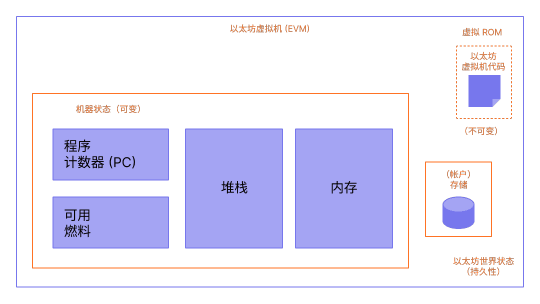
\includegraphics[width=.3\linewidth]{pictures/ethereum_solidity_version_history}
    \caption{\label{fig:ethereum_solidity_version_history}以太坊和Solidity自2019年以来的版本更迭}
\end{figure}
下一步是确定搜集何种数据以及如何搜集数据。本文的目标是研究智能合约的漏洞情况,以及在以太坊虚拟机上的执行情况,因此需要从以太坊网络获取至少产生过一笔交易的智能合约。相比于Github等代码托管平台上的智能合约源代码,从以太坊区块链上获取的智能合约更加具有现实意义。Evgeny\cite{bigquery_ethereum}在BigQuery\footnote{Google BigQuery 是 Google Cloud Platform 提供的一项企业级数据仓库服务,它允许执行快速的 SQL 查询和交互式分析大规模数据集}上创建并公开了以太坊数据库,包含以太坊区块链上智能合约和交易的所有信息。同时部署了自动化工具每天从以太坊中提取最新的数据,并将其同步到数据库中。另一方面,Etherscan\footnote{Etherscan的网址}是一个以太坊区块链数据分析平台,提供了应用程序接口(Application Programming Interface,API)用于查询区块链上的数据。综上所述,搜集数据的方法包含2个步骤:首先使用BigQuery数据库收集至少有一笔交易的智能合约账户地址,然后将合约地址作为参数调用Etherscan相关的API得到智能合约的源代码等数据。
\subsection{数据预处理}
\label{sec:数据预处理}

最后一步需要对原始数据集进行预处理,过滤掉一些不符合期望的智能合约,我们设定了以下的排除规则:
\begin{enumerate}
    \item \textbf{移除重复的合约}。有些合约可能会被重复部署,所以我们比较Solidity文件的MD5值,如果相同则排除其一。
    \item \textbf{移除交易数太少的合约}。交易数太少的合约可能含有严重的缺陷,没有足够的运行信息证明其安全性,所以研究意义不大。
    \item \textbf{移除编译错误的合约}。编译错误的合约无法运行,没有研究价值。
    \item \textbf{移除低版本的合约}。低于0.4.11的Solidity版本与更新版本存在较大差异,且可能在将来被废弃。
\end{enumerate}

通过上述方法,我们首先在BigQuery中得到了xxx个智能合约地址,在Etherscan上获得的经过验证的合约源代码共有xxx份,最后经过上述排除规则,我们总计得到了xxx份智能合约源代码用于下文的研究。
\subsection{数据打标签}
\label{sec:数据打标签}
\textcolor{red}{这里可能要给数据集打标签}
\section{基于静态度量定义专家特征}
\label{sec:基于静态度量定义专家特征}
在软件质量保证(Software Quality Assurance,SQA)工作中,静态代码指标(如 Halstead\cite{halstead}指标、McCabe\cite{mccabe}指标)发挥着重要作用。许多方法都是基于静态代码指标提出的,先前的工作\cite{menzies2007data,meyers2007empirical,zimmermann2007predicting}也证实了这些指标对软件质量保证研究是有用的。因此,我们认为智能合约也可以从中获益,借助静态代码指标对合约进行漏洞检测和运行时崩溃研究。

受先前工作\cite{halstead,mccabe,menzies2007data}的启发,本文定义了34个静态代码指标,其中22个与编程语言无关,这些指标进一步分为三个维度:复杂度度量指标、计数度量指标和面向对象度量指标;另外12个为Solidity语言相关的度量指标,这是因为智能合约与其他传统语言编写的程序有所不同,一些特性(如Gas机制)相关的指标可能会更精准地表征一个智能合约。

% 表\autoref{tab:metrics}显示了本文引入或定义的静态代码指标的概述,具体每个指标的含义将在下一小节阐述。

% \begin{table}[htbp]
%     \caption{\label{tab:metrics}本文引入或定义的静态代码指标}
%     \small
%             \renewcommand{\arraystretch}{1.5}
%         \begin{tabularx}{\linewidth}{cX<{\raggedright}X<{\raggedright}}
%             \hline
%             \textbf{Dimension}            & \textbf{Metric}              & \textbf{Description} \\ \hline
%             \multirow{6}{*}{代码复杂度指标} & 平均圈复杂度(AvgComplexity)        & 所有嵌套函数的平均严格圈复杂度 \\
%                                        & 最大圈复杂度(MaxComplexity)        & 严格圈复杂度的最大值 \\
%                                        & 最大继承深度(MaxInheritance)   & 合约继承树的最大深度 \\
%                                        & 最大嵌套度(MaxNesting)           & 控制结构的最深嵌套级别 \\
%                                        & 圈复杂度总和(SumComplexity)        & 所有嵌套函数的严格圈复杂度之和 \\
%                                        & 合约耦合度(CountContractCoupled)  & 与当前合约存在耦合关系的合约数量 \\ \hline
%             \multirow{6}{*}{计数度量} & 代码行数(CountLineCode)       & Solidity 源代码文件的总行数 \\
%                                        & 可执行代码行数(CountLineCodeExe)     &  Solidity 源代码文件中的非空行和非注释行 \\
%                                        & 注释行数(CountLineComment)     & Solidity 源代码文件中注释的总行数 \\
%                                        & 语句数(CountStmt)            &  Solidity 源代码文件中可执行语句的数量 \\
%                                        & 空行数(CountLineBlank)       & Solidity 源代码文件中的空行数 \\
%                                        & 注释代码行数比(RatioCommentToCode)   & Solidity 源代码文件中注释行数与代码行数的比值 \\ \hline
%             \multirow{10}{*}{面向对象维度} & 父合约个数(CountContractBase)    &  Solidity 文件中的主合约所继承的合约的数量 \\
%                                        & 依赖合约个数(CountDependence)      & 直接依赖继承的父合约与间接依赖的父合约继承的合约总数 \\
%                                        & 合约个数(CountContract)        & Solidity 源文件中定义的合约的数量 \\
%                                        & 函数总数(CountTotalFunction)   & Number of stract functions including modifier functions. \\
%                                        & 公共变量个数(CountFunctionPublic)  & Number of public variables. \\
%                                        & 变量个数(CountVariable)        & Number of contract variables. \\
%                                        & 私有函数个数(CountFunctionPrivate) & Number of private functions. \\
%                                        & 内部函数个数(CountFunctionInternal) & Number of internal functions. \\
%                                        & 外部函数个数(CountFunctionExternal) & Number of external functions. \\
%                                        & 公开函数个数(CountPublicVariable)  & Number of public functions. \\ \hline
%             \multirow{12}{*}{Solidity维度} & 接口数量(NOI)                 & Solidity 源文件中使用的接口总数 \\
%                                        & 依赖库数量(NOL)                & Solidity 源文件中使用的库总数\\
%                                        & 存储变量数(NOSV)                & 定义的存储变量总数 \\
%                                        & 映射变量数(NOMap)              & 使用的映射类型总数 \\
%                                        & 可支付函数数量(NOPay)               & Solidity 源文件中调用的可支付函数总数 \\
%                                        & 事件数量(NOE)                 & Solidity 源文件中发生的事件总数 \\
%                                        & 函数修改器数量(NOMod)               &  Solidity 源文件中调用的修改器总数 \\
%                                        & 转账语句数(NOT)                 & 所有函数中执行的转账语句总数 \\
%                                        & 信息调用数(NOC)                 & Solidity 源文件中消息调用次数总数 \\
%                                        & 委托调用数(NODC)                & 所有函数中执行的委托调用总数 \\
%                                        & 静态函数数量(NOSF)                & 静态函数数量,包括视图函数和纯函数 \\
%                                        & 重写回调函数(SDFB)                & Solidity 源文件中是否重写了 fallback 函数 \\ \hline
%         \end{tabularx}
% \end{table}
% \subsection{静态代码度量的四个维度}
\label{sec:静态代码度量的四个维度}
\subsection{代码复杂度}
\label{sec:代码复杂度}

代码复杂度指标(Code Complexity Metrics)是用于量化软件源代码复杂性的度量标准。有研究表明\cite{Chen2019AnEI,singh2015bug},代码复杂度指标与程序中的复杂缺陷存在一定的相关性,这些指标可用于评估代码的难以理解性、可维护性和潜在缺陷。直观地说,一段代码越复杂,它成为缺陷代码的概率就越高,因此可以利用代码复杂度指标建立缺陷预测模型。

本文结合已有工作,引入了关于Solidity文件的6个复杂度指标:平均圈复杂度、最大圈复杂度、圈复杂度总和、最大继承深度、最大嵌套度、合约耦合度。
\begin{enumerate}[label=\Alph*., align=left, leftmargin=*]
    \item \textbf{平均圈复杂度(AvgComplexity)\&最大圈复杂度(MaxComplexity)\&圈复杂度总和(SumComplexity)}。
    圈复杂度用来衡量一个程序判定结构的复杂程度,在数量上表现为程序中可以独立执行的路径条数。我们从两个方面计算圈复杂度:1) 遍历并统计抽象语法树上相应函数节点下的所有分支语句(如 if、while、do while 和 for 等);2)计算源代码文件中"\&\&"、"||"和"? : "的总数。因此,Solidity文件中的最大圈复杂度就是所有函数的圈复杂度的最大值,圈复杂度总和就是所有函数的圈复杂度之和,平均圈复杂度就是所有函数的圈复杂度之和与函数个数的比值。
    \item \textbf{最大继承深度(MaxInheritance)}。
    Solidity作为面向对象的编程语言,合约之间可以存在继承关系,合约的最大继承深度表示当前合约在所有继承链(因为Solidity支持多重继承)中的路径长度。一个 Solidity 文件中可能有多个合约,但只有一个合约是主合约(类似于Java文件中的公开类),其他合约都是辅助合约或继承合约,因此该指标计算的是主合约的最大继承深度。我们采用递归算法来计算这一指标,即当前合约的继承深度为父合约的继承深度值加1,如果某个合约没有父合约,则它的继承深度值为0。
    \item \textbf{最大嵌套度(MaxNesting)}。
    最大嵌套度表示 Solidity 文件中函数内控制结构的最深嵌套级别。要计算单个函数的嵌套级别,我们需要遍历该函数中的所有语句,并计算从语句到函数定义的路径上分支语句的数量。因此,Solidity 文件的最大嵌套度为函数中的语句嵌套度中的最大值。
    \item \textbf{合约耦合度(CountContractCoupled)}。
    合约耦合度指标衡量的是与当前合约存在耦合关系的合约数量。当一个合约的函数调用另一个合约的函数或访问另一个合约的变量时,我们认为这两个合约是耦合的。这个指标用来反映合约之间的关联情况,并反映某个合约使用了多少其他类型的合约(如作为状态变量类型、局部变量类型、函数参数等)。我们将引用合约 C1 或被它引用的其他合约集合的大小作为合约 C1 的合约耦合度。
\end{enumerate}
\subsection{计数维度}
\label{sec:计数维度}
计数度量(Count Metrics)用于从物理层面(如代码行数、空行数或注释行数)来表示代码特征,Gyimothy 等人\cite{gyimothy2005}证实了计数相关的指标在缺陷预测工作中的实用性。直观地说,一个程序的代码量越大,出现缺陷代码的概率就越高。本文引入了6个计数相关的度量指标:代码行数、可执行代码行数、注释行数、语句数、空行数、注释代码行数比。
\begin{enumerate}[label=\Alph*., align=left, leftmargin=*]
    \item \textbf{代码行数(CountLineCode)}。即Solidity源代码文件的总行数。

    \item \textbf{可执行代码行数(CountLineCodeExe)}。可执行代码行数指标计算的是 Solidity 源代码文件中的非空行和非注释行。也就是说,只计算包含实际Solidity语句的行数。为了计算这个指标,我们逐行扫描源代码,过滤掉所有空行和注释行,得到 CountLineCodeExe 指标。在 Solidity 编程语言中,有两种注释源代码的方法:单行注释("//")和多行注释("/*...*/")。因此,我们认为所有以"/*"、"*"、"//"开头或以 "*/"结尾的行都是注释行。
    
    \item \textbf{注释行数(CountLineComment)}。该指标可以在上述可执行代码行数指标的计算过程中得到。
    
    \item \textbf{语句数(CountStmt)}。即 Solidity 源代码文件中可执行语句的数量,可以从 Solidity 源代码对应的抽象语法树中计算语句定义的数量得到。
    
    \item \textbf{空行数(CountLineBlank)}。即 Solidity 源代码文件中的空行数。
    
    \item \textbf{注释代码行数比(RatioCommentToCode)}。即 Solidity 源代码文件中注释行数与代码行数的比值。
\end{enumerate}
\subsection{面向对象维度}
\label{sec:面向对象维度}
面向对象的度量指标用于从高层次角度描述源代码的质量。面向对象设计思想的核心是用对象来模拟现实世界,这与强调面向函数的、将数据和程序分开的传统程序设计方式截然不同。先前的工作\cite{martin1994oodesign,basili1996validation,KHAN20071}证实了面向对象度量指标在缺陷预测工作中比传统指标(如代码复杂度指标、计数指标)更有效。
\begin{enumerate}[label=\Alph*., align=left, leftmargin=*]
    \item \textbf{父合约个数(CountContractBase)}。即Solidity文件中的主合约所继承的合约的数量。

    \item \textbf{依赖合约个数(CountDependence)}。主合约除了直接依赖继承的父合约外,还间接依赖父合约所继承的合约,因此该指标计算两种合约的总数。

    \item \textbf{合约个数(CountContract)}。即Solidity源文件中定义的合约的数量。

    \item \textbf{内部函数个数(CountFunctionInternal) \& 外部函数个数(CountFunctionExternal) \& 私有函数个数(CountFunctionPrivate) \& 公开函数个数(CountFunctionPublic) \& 函数总数(CountTotalFunction)}。 在 Solidity 语言中,函数和状态变量有四种可见性:外部、内部、公开和私有,合约中定义的函数必须指定为这四种类型之一。然而,对于状态变量,外部函数是不可能的。外部函数是合约接口的一部分,这意味着它们只能从其他合约或通过事务调用。公共函数也是合约接口的一部分,可以在内部调用,也可以通过消息调用。对于公共状态变量,会在合约中生成一个自动获取函数。对于内部函数和状态变量,它们只能在内部被访问(即在当前合约或派生合约内)。对于私有函数和状态变量,它们只能在定义它们的合约中可见,而不能在派生合约中可见。为了计算 Solidity 源代码文件中的这些指标,我们会根据抽象语法树中的函数节点,总结出外部、公共、内部或私有函数定义的相应数量。
    在 Solidity 语言中,函数和状态变量有四种和三种可见性类型,分别是:外部(external)、内部(internal)、公开(public)和私有(private)。合约中定义的函数必须指定为这四种类型之一。然而,对于状态变量,它们不能被标记为外部(external)类型。外部函数是合约接口的一部分,这意味着它们只能从合约外部被调用,包括其他合约或通过交易。公开函数也是合约接口的一部分,它们既可以在合约内部被调用,也可以从外部通过交易调用。对于标记为公开的状态变量,Solidity 会在合约中自动生成一个相应的获取器函数(getter)。内部函数和状态变量只能在当前合约或其派生合约内被访问。而私有的函数和状态变量则仅在其定义的那个合约中可见,不能在派生合约中被访问。我们通过解析抽象语法树(AST)中的节点信息来分析这些不同类型的函数和状态变量。
    \item \textbf{变量个数(CountVariable)\& 公共变量个数(CountPublicVariable)}。即Solidity源文件中的所有合约中的变量个数和被标记为公共变量的个数。
\end{enumerate}
\subsection{Solidity维度}
\label{sec:Solidity维度}
不同编程语言的特性对代码质量的影响各不相同, Solidity 作为一种专为智能合约设计的编程语言更是如此,其特性包括:全局状态、事件机制、Gas机制等。鉴于智能合约的这些特性,我们提出了针对Solidity语言的一系列启发式指标。

智能合约的设计目标是运行在以太坊网络节点的虚拟机上,因此其执行过程中对各种资源极为敏感,这也突出了Gas机制的重要性。在以太坊网络中,几乎所有智能合约操作均需消耗Gas,比如资金转移、数据存储、调用其他智能合约或记录运行日志等,不同操作消耗的Gas数量各不相同。因此,智能合约中的操作越多,消耗的Gas也就越多,进而增加合约因Gas耗尽而崩溃的风险。基于此,我们定义了八个度量指标:存储变量数、映射变量数、可支付函数数量、事件数量、函数修改器数量、转账语句数量、调用语句数量、代理调用语句数量。

由于以太坊区块链的不可变性,部署在以太坊上的智能合约代码无法修改,即使存在错误或被其他合约所依赖,这一特性可能增加合约在执行过程中崩溃的风险。为此,我们定义了两个指标用于描述这种特性:静态函数数量、依赖库数量。

同时,我们认为良好的代码结构(例如模块化)对代码可读性和质量有重要影响。因此,我们引入了接口数量指标来评估代码结构的优劣。

总体而言,我们提出了12个Solidity特有的度量指标,下文将深入解析这些指标的含义和作用。

\begin{enumerate}[label=\Alph*., align=left, leftmargin=*]
    \item \textbf{存储变量数(NOSV)}。以太坊虚拟机有三个可以存储数据的区域:storage、内存和堆栈。以太坊的每个账户都有一个名为 "storage"的数据区,它在函数调用和交易之间是持久的。不过,读取和写入的成本较高。存储变量数指标衡量的是 Solidity 源代码文件中定义了多少个存储在storage的变量。此外,有三种数据类型(即映射、数组和结构体)默认为storage类型的变量。定义的storage变量越多,执行该合约消耗的Gas也就越多,智能合约崩溃的概率就越高。
    \item \textbf{映射变量数(NOMap)}。映射类型(Mapping)是 Solidity 编程语言中最常用的数据类型之一,支持存储键值对,类似于哈希表。但是,映射类型的key只能是基本数据类型,也没有内部变量记录元素的个数,而且也不支持像 "foreach循环"操作那样访问所有元素。因此,这种类型的变量会因为其诸多限制\footnote{由于原生的 Mapping 限制比较多,以太坊官方提供了一个扩展库 IterableMapping ,https://github.com/ethereum/dapp-bin/blob/master/library/iterable\_mapping.sol,增加了类似其他语言的映射类型的操作。}而增加智能合约漏洞和崩溃的风险。
    \item \textbf{可支付函数数量(NOPay)}。可支付函数(Payable Function)提供了接收资金(以太币)转移的功能。然而,成功支付至少需要两个基本条件:发送方具有足够的Gas以及有效的接收方地址。因此,如果不满足这两个条件,合约运行中就会崩溃。可支付函数数量指标衡量 Solidity 源代码文件中定义了多少个可支付函数。
    \item \textbf{事件数量(NOE)}。Solidity 中的事件是对以太坊虚拟机日志功能的封装。应用程序可以通过以太坊客户端的 RPC 接口订阅并监听这些事件,以获取相应的消息。然而,事件也需要Gas来驱动。事件的使用量越多,Gas的消耗量就越大。
    \item \textbf{函数修改器数量(NOMod)}。修改器是函数的包装器,可以以声明的方式改变函数的行为。例如,我们可以使用修改器在执行特定函数之前做条件检查,当然这需要消耗Gas。
    \item \textbf{转账语句数(NOT)}。transfer是address类型数据的原生属性,用于向该地址对应的账户转账。调用transfer后会调用转账接收方的fallback函数,如果该函数逻辑太复杂会导致transfer执行失败,因此转账语句越多,合约运行崩溃的概率也就越高。
    \item \textbf{消息调用数(NOC)}。消息调用(Message Call)用于智能合约之间的交互,进行消息调用需要提供源地址、目标地址、数据、以太币、Gas,发起一笔交易、调用其他合约的函数或者发送以太币到非合约账户都是消息调用,消息调用次数越多,合约出现运行异常的概率越高。
    \item \textbf{委托调用数(NODC)}。消息调用有一种变体——委托调用(Delegate Call),它与消息调用的不同之处在于,目标地址的代码将在发起调用的合约的上下文中执行。这意味着一个合约可以在运行时从另外一个地址动态加载代码,storage、当前地址和余额都指向发起调用的合约,只有代码是从被调用地址获取的。委托调用可能会从被调用合约引入漏洞,因此该指标是有意义的。
    \item \textbf{静态函数数量(NOSF)}。静态函数是指那些保证不会读取或修改状态变量的函数,在 Solidity 中用pure或view关键字修饰。
    \item \textbf{重写回调函数(SDFB)}。当调用的函数签名与合约中任何函数都不匹配时,默认调用 fallback 函数。最好重新写fallback函数以应对未知的调用,同时使用 payable 修饰以接收转账,该指标表示是否重写了fallback函数。
    \item \textbf{依赖库数量(NOL)}。库(Library)是一种特殊的合约,其中的函数必须保证不修改状态。库被部署在特定地址后可以重复使用。然而库的质量直接影响了主合约的质量,如果库中存在分享代码,依赖它的智能合约就会包含潜在风险。该指标衡量了Solidity源文件中使用了多少库。
    \item \textbf{接口数量(NOI)}。良好的结构设计可以提高代码质量,接口(Interfact)将类的定义与实现分离开来,提供了更好的可读性和可扩展性。因此,使用接口进行模块化设计可以在一定程度上提高合约质量。
\end{enumerate}

\section{基于合约语义图提取语义特征}
\label{sec:基于合约语义图提取语义特征}
%描述一下语义信息对深度学习的意义。

已有许多工作证明,相比于源代码,基于图的表示法往往更能保留复杂程序的结构特征\cite{allamanis2017learning},这有助于模型更好地理解程序的语义信息,从而提高在代码理解相关下游任务中的性能。这些与程序结构相关的图称为语义图(Semantic Graph),应用最广泛的语义图便是抽象语法树,此外还有数据流图、控制流图、函数调用图等。本文拟挖掘智能合约中的语义信息用于训练缺陷检测模型,因此在此章节引入智能合约的数据流图、控制流图和函数调用图,下面将介绍一下这三种语义图及其从智能合约源代码中的构建方法。

\subsection{数据流图}
\label{sec:数据流图}
数据流图(Data Flow Graph,DFG)是一种表示变量之间依赖关系的有向图,其中节点表示变量,有向边表示变量值的流动方向。数据流图为模型理解程序的结构特征带来了关键的语义信息,已被广泛应用在各种程序分析工作中\cite{hellendoorn2019global,allamanis2018learning,guo2020graphcodebert}。

与AST不同的是,对于相同功能的程序,尽管各种语言的抽象语法不同,但数据流是相同的。以 $a=maxValue-minValue$ 为例,仅从变量a的名字是无法得知该变量值所代表的实际含义,但从数据流的角度来看,a的值来自maxValue和minValue的差,变量a的含义可能是一个数组的极差。

另一方面,数据流图的引入可以让模型更加关注变量之间的直接依赖关系。以图xxx为例,有四个名称相同但语义不同的变量(x1,x2,x3,x4),图中展示了这些变量之间的依赖关系,并表明x4与x3的关系相比于x2更加紧密,这样就极有可能让模型更加关注变量x3的值,从而发现潜在的漏洞。
如果用形式化语言表述,将从AST中得到的变量序列记为$V=\left\{v_1, v_2, \ldots, v_k\right\}$,将表明了数据流动方向的边的集合表示为$E=\left\{\varepsilon_1, \varepsilon_2, \ldots, \varepsilon_l\right\}$,那么图$\mathcal{G}(C)=(V, E)$表示源代码$C$中的数据流图。
%%%%%%%%%%%%%%%%%%%% 如果需要时再增加这部分内容 %%%%%%%%%%%%%%%
Wu等人在研究智能合约的重入漏洞时,提出了关键数据流图(Curcial Graph Flow Data,CDFG)的概念\cite{wu2021peculiar}。他们认为,智能合约的漏洞存在于几个关键语句中,整个数据流图中也只有部分信息对于漏洞检测任务有帮助。因此为了减少无用信息的干扰,他们通过剔除DFG中与漏洞无关的数据流关系,构建了关键数据流图,用来表达合约中与漏洞相关的关键语义信息。本文将沿用其思路与做法。
\subsection{控制流图}
\label{sec:控制流图}

控制流图(Control Flow Graph,CFG)是一个过程或程序逻辑的抽象表示,描述了程序在执行期间可能经过的所有路径。Allen于1970年提出控制流图的概念\cite{allencfg},后来逐渐成为静态分析和编译器优化的重要工具。

在控制流图中,节点表示一个基本代码块,既没有任何跳转指令的顺序执行的代码块,有向边表示程序的执行路径,在满足一定条件时,程序从一个基本代码块跳转到另一个基本代码块继续执行。

控制流图对应的是代码中的条件分支结构,在大多数高级编程语言中用if-else语句、while语句、for语句等表示。图xx表示了

构建控制流图的方法:
\subsection{函数调用图}
\label{sec:函数调用图}
函数调用图(Call Graph)是描述程序中函数互相调用关系的有向图,这是一种特殊的控制流图,其分支逻辑由函数调用实现。

在函数调用图中,每个节点均表示一个函数,有向边表示起点函数调用了终点函数。

构建函数调用图的方法



